% fig11-trust-boundary.tex — Figure 11: Trust boundaries (DEV-GOV-03)
%
% What Sego asserts, what it observes, and what it must treat as an untrusted
% claim. The figure exists because the three are easy to read as one: a value that
% Sego observed with its own eyes and a value a model reported are drawn on
% different sides of a line here.
%
% The trust model itself is model-assisted: nothing in this picture is a
% cryptographic proof of provenance.
\documentclass[tikz,border=10pt]{standalone}
\usetikzlibrary{arrows.meta,positioning,fit,backgrounds,calc}

\begin{document}
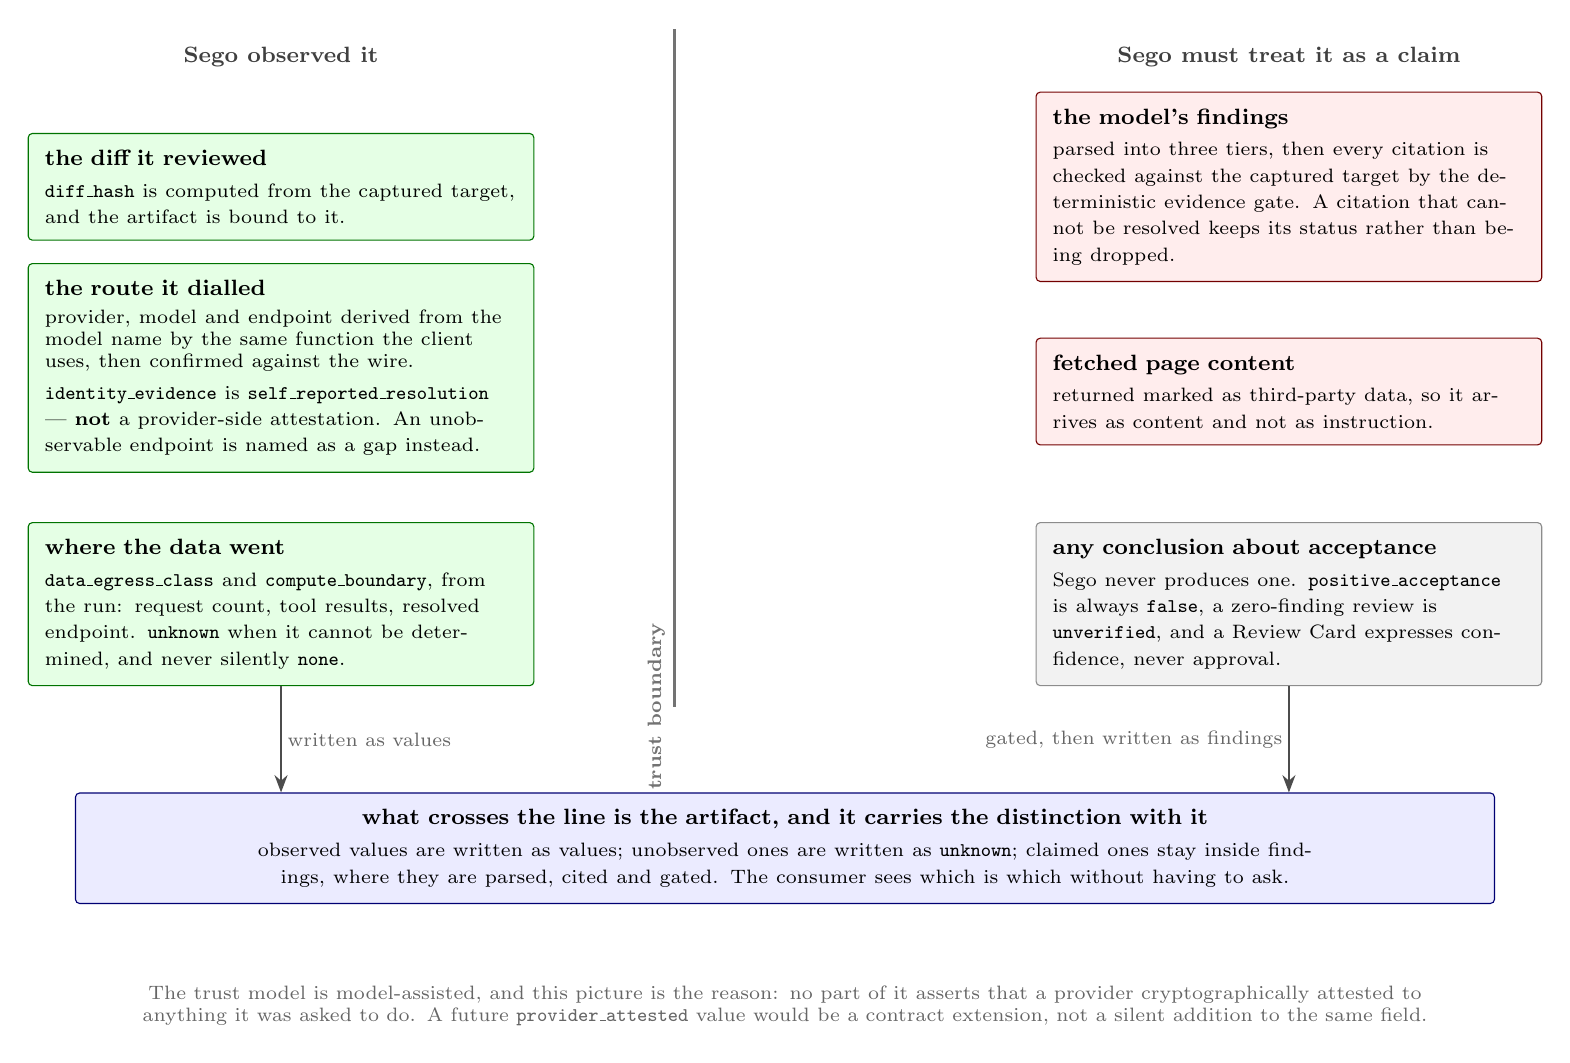
\begin{tikzpicture}[
  x=1cm, y=1cm,
  font=\small,
  band/.style={draw, rounded corners=1.5pt, font=\footnotesize,
               align=left, inner sep=6pt, text width=60mm},
  obs/.style={band, fill=green!10, draw=green!45!black},
  claim/.style={band, fill=red!7, draw=red!45!black},
  never/.style={band, fill=black!5, draw=black!45},
  arr/.style={-{Stealth[length=2.2mm]}, thick, draw=black!70},
  bar/.style={draw=black!55, line width=1.2pt},
  lab/.style={font=\scriptsize, text=black!60, inner sep=2pt, fill=white},
  hdr/.style={font=\footnotesize\bfseries, text=black!75, anchor=south}
]

% ---------------- observed ----------------
\node[hdr] at (-6.4, 5.4) {Sego observed it};
\node[obs] (owndiff) at (-6.4, 4.0)
  {\textbf{the diff it reviewed}\\[2pt] \scriptsize \texttt{diff\_hash} is computed from the captured target, and the
   artifact is bound to it.};
\node[obs] (route) at (-6.4, 1.7)
  {\textbf{the route it dialled}\\[2pt] \scriptsize provider, model and endpoint derived from the model name by the
   same function the client uses, then confirmed against the wire.\\[2pt]
   \scriptsize \texttt{identity\_evidence} is \texttt{self\_reported\_resolution} --- \textbf{not} a provider-side
   attestation. An unobservable endpoint is named as a gap instead.};
\node[obs] (egress) at (-6.4, -1.3)
  {\textbf{where the data went}\\[2pt] \scriptsize \texttt{data\_egress\_class} and \texttt{compute\_boundary}, from the
   run: request count, tool results, resolved endpoint. \texttt{unknown} when it cannot be determined, and never
   silently \texttt{none}.};

% ---------------- claims ----------------
\node[hdr] at (6.4, 5.4) {Sego must treat it as a claim};
\node[claim] (model) at (6.4, 4.0)
  {\textbf{the model's findings}\\[2pt] \scriptsize parsed into three tiers, then every citation is checked against
   the captured target by the deterministic evidence gate. A citation that cannot be resolved keeps its status
   rather than being dropped.};
\node[claim] (web2) at (6.4, 1.4)
  {\textbf{fetched page content}\\[2pt] \scriptsize returned marked as third-party data, so it arrives as content
   and not as instruction.};
\node[never] (verdict) at (6.4, -1.3)
  {\textbf{any conclusion about acceptance}\\[2pt] \scriptsize Sego never produces one. \texttt{positive\_acceptance}
   is always \texttt{false}, a zero-finding review is \texttt{unverified}, and a Review Card expresses confidence,
   never approval.};

% ---------------- the line ----------------
\draw[bar] (-1.4, 6.0) -- (-1.4, -2.6);
\node[font=\scriptsize\bfseries, text=black!55, rotate=90, anchor=south] at (-1.4, -2.6)
  {trust boundary};

% ---------------- the artefact crosses ----------------
\node[band, fill=blue!8, draw=blue!45!black, text width=176mm, align=center] (out) at (0, -4.4)
  {\textbf{what crosses the line is the artifact, and it carries the distinction with it}\\[2pt]
   \scriptsize observed values are written as values; unobserved ones are written as \texttt{unknown}; claimed ones stay
   inside findings, where they are parsed, cited and gated. The consumer sees which is which without having to ask.};

% Short vertical drops from the two lowest boxes. Long diagonals from the top
% boxes to the band crossed every box in between.
\draw[arr] (egress.south) -- node[lab, right] {written as values} (out.north -| egress);
\draw[arr] (verdict.south) -- node[lab, left] {gated, then written as findings} (out.north -| verdict);

\node[font=\scriptsize, text=black!60, text width=182mm, align=center] at (0, -6.4)
  {The trust model is model-assisted, and this picture is the reason: no part of it asserts that a provider
   cryptographically attested to anything it was asked to do. A future \texttt{provider\_attested} value would be a contract
   extension, not a silent addition to the same field.};

\end{tikzpicture}
\end{document}
